\documentclass[[12pt,twoside]{book}
\usepackage{_my_document_style}
\begin{document}
%
\def\myAhaI{999}
\def\myMach{0.4}
\def\myStartSurveyAircraftWingData{-999}
\def\myAhaII{999}
\def\myAreaWingMTsquared{28}
\def\myAreaWingFTsquared{301.39}
\def\mySpanWingMT{16}
\def\mySpanWingFT{52.49344}
\def\myTaperRatioWing{0.4}
\def\myInducedDragFactorWing{0.9}
\def\mySweepLEWingRAD{0}
\def\mySweepLEWingDEG{0}
\def\mySweepQuarterChordWingRAD{-0.04684}
\def\mySweepQuarterChordWingDEG{-2.684}
\def\mySweepHalfChordWingRAD{-0.09348}
\def\mySweepHalfChordWingDEG{-5.356}
\def\mySweepTEWingRAD{-0.18535}
\def\mySweepTEWingDEG{-10.62}
\def\myTwistWingRAD{-0.04363}
\def\myTwistWingDEG{-2.5}
\def\myAlphaZeroLiftRootWingRAD{-0.05236}
\def\myAlphaZeroLiftRootWingDEG{-3}
\def\myAlphaZeroLiftTipWingRAD{-0.02618}
\def\myAlphaZeroLiftTipWingDEG{-1.5}
\def\myAlphaZeroLiftMeanWingRAD{-0.04114}
\def\myAlphaZeroLiftMeanWingDEG{-2.4}
\def\myThicknessOverChordRootWing{0.15}
\def\myThicknessOverChordTipWing{0.09}
\def\myThicknessOverChordMeanWing{0.124}
\def\myCmZeroRootWing{-0.08}
\def\myCmZeroTipWing{-0.1}
\def\myCmZeroMeanWing{-0.0885714}
\def\myCLAlphaRootWingRAD{6.15}
\def\myCLAlphaRootWingDEG{0.10734}
\def\myCLAlphaTipWingRAD{6.05}
\def\myCLAlphaTipWingDEG{0.10559}
\def\myCLAlphaMeanWingRAD{6.10714}
\def\myCLAlphaMeanWingDEG{0.10659}
\def\myPrepareForStackNull{-1e+307}
\def\myChordRootWingMT{2.5}
\def\myChordRootWingFT{8.2}
\def\myChordTipWingMT{1}
\def\myChordTipWingFT{3.28}
\def\myXsiacRootWing{0.25}
\def\myXsiacTipWing{0.25}
\def\myAhaII{999}
\def\myCoeffATwistWingRADMT{-0.005454}
\def\myCoeffATwistWingDEGMT{-0.3125}
\def\myCoeffATwistWingRADFT{-0.0016624}
\def\myCoeffATwistWingDEGFT{-0.09525}
\def\myCoeffBTwistWingRAD{0}
\def\myCoeffBTwistWingDEG{0}
\def\myCoeffAChordWing{-0.1875}
\def\myCoeffBChordWingMT{2.5}
\def\myCoeffBChordWingFT{8.2021}
\def\myCoeffAAeroTwistWingRADMT{0.003272}
\def\myCoeffAAeroTwistWingDEGMT{0.1875}
\def\myCoeffAAeroTwistWingRADFT{0.0009975}
\def\myCoeffAAeroTwistWingDEGFT{0.05715}
\def\myCoeffBAeroTwistWingRAD{-0.05236}
\def\myCoeffBAeroTwistWingDEG{-3}
\def\myCoeffAPercThicknessWingMT{-0.0075}
\def\myCoeffAPercThicknessWingFT{-0.002286}
\def\myCoeffBPercThicknessWing{0.15}
\def\myCoeffAClalphaWingRADMT{-0.0125}
\def\myCoeffAClalphaWingRADFT{-0.00381}
\def\myCoeffAClalphaWingDEGMT{-0.0002182}
\def\myCoeffAClalphaWingDEGFT{-6.65e-05}
\def\myCoeffBClalphaWingRAD{6.15}
\def\myCoeffBClalphaWingDEG{352.369}
\def\myCoeffACmZeroWingMT{-0.0025}
\def\myCoeffACmZeroWingFT{-0.000762}
\def\myCoeffBCmZeroWing{-0.08}
\def\myCoeffAXsiACWingMT{0}
\def\myCoeffAXsiACWingFT{0}
\def\myCoeffBXsiACWing{0.25}
\def\myAhaII{999}
\def\myAspectRatioWing{9.143}
\def\myMACWingMT{1.86}
\def\myMACWingFT{6.09}
\def\myAlphaZeroLiftWingRAD{-0.02244}
\def\myAlphaZeroLiftWingDEG{-1.286}
\def\myCLAlphaWingRAD{4.94007}
\def\myCLAlphaWingDEG{0.0862205}
\def\myCmZeroAWing{-0.0873077}
\def\myCmZeroBWing{-0.0037723}
\def\myCmZeroWing{-0.09108}
\def\myXMACLEToApexWingMT{0}
\def\myXMACLEToApexWingFT{0}
\def\myYMACWingMT{3.43}
\def\myYMACWingFT{11.25}
\def\myACWingToMACLEWingMT{0.43856}
\def\myACWingToMACLEWingFT{1.43884}
\def\myACWingToApexWingMT{0.43856}
\def\myACWingToApexWingFT{1.43884}
\def\myXsiACWing{0.23615}
\def\myKOneACDatcomWing{1.34174}
\def\myKTwoACDatcomWing{0}
\def\myXACOverChordRootDatcomWing{0.176}
\def\myAhaII{999}
\def\myAhaII{999}
\def\myAhaII{999}
\def\myAhaII{999}
\def\myAhaII{999}
\def\myAhaII{999}

%
\begin{myExampleX}{Pitching moment around the wing aerodynamic center}{\ding{46}}% \ \Keyboard\ %
\label{example:Wing:Cmac:B}
%
\noindent
The example~\ref{example:Wing:Cmac:A} (see figure~\ref{fig:Wing:Cmac:Results:A}) is taken up here considering
a more accurate law of basic loading.
It was obtained numerically and is plotted in the figure~\ref{fig:Wing:Cmac:Results:BA}.
The numerical values are shown in the table~\ref{tab:Wing:Cmac:Results:B}.
%
In the figure~\ref{fig:Wing:Cmac:Results:BB} the function is compared
$(cC_\ell)_\mathrm{b,Schrenk}(Y)$, obtained in conjunction with the application of the Schrenk engineering method for the additional loading (see example~\ref{example:Wing:Cmac:A}),
with function $(cC_\ell)_\mathrm{b}(Y)$, which interpolates a sequence of discrete values
obtained by applying Prandtl's Lifting Line Theory.

\begin{table}[tb]
\caption{%
 Wing assigned in the examples~\ref{example:Wing:Cmac:A} e ~\ref{example:Wing:Cmac:B}.
Numerical values with which the basic loading was calculated $(cC_\ell)_\mathrm{b}$ 
  applying Prandtl's Lifting Line Theory..
}
\label{tab:Wing:Cmac:Results:B}
\centering
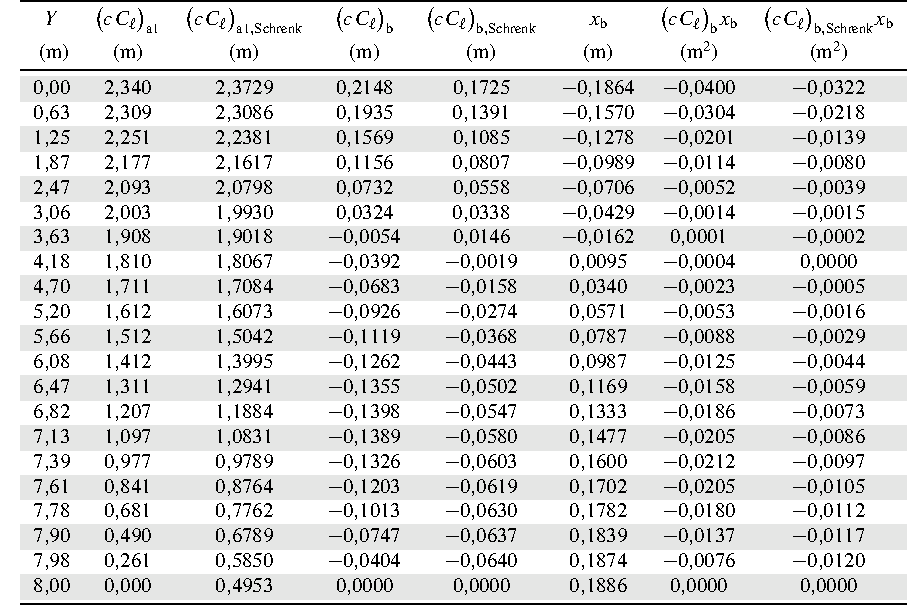
\includegraphics[width=0.95\textwidth]{Chapter_2/pitching_moment_two/wing_Cmac_2_loading_table.pdf}
\end{table}

In the case discussed here the function $x_\mathrm{b}(Y)$ and the valute of
 $C_{\mathcal{M}_\mathlarger{\mathrm{ac,b}}}$ coincide with what was obtained
in the example~\ref{example:Wing:Cmac:A}.
As for the value of $C_{\mathcal{M}_\mathlarger{\mathrm{ac,b}}}$, having a more accurate trend of the basic loading, a different value is obtained

\[
C_{\mathcal{M}_\mathlarger{\mathrm{ac,b}}} 
  =
  \frac{2}{S\,\bar{c}} \int_0^{b/2} \big(cC_{\ell}\big)_\mathrm{b}(Y) \; x_\mathrm{b}(Y)\, \diff{Y}
  = 
  \mathunderline{mydarkblue}{ \SI[round-precision=5]{\myCmZeroBWing}{} }
\]
The integral in this formula was evaluated numerically after defining a function
interpolating $(cC_\ell)_\mathrm{b}(Y)$ piecewise linear in the interval
$[0,\frac{1}{2}b]$.
The figure~\ref{fig:Wing:Cmac:Results:BC} plot the discrete values of the
integrating function
%$\big(cC_{\ell}\big)_\mathrm{b}(Y) \, x_\mathrm{b}(Y)$,
$\big(cC_{\ell}\big)_\mathrm{b} \, x_\mathrm{b}$,
already listed in the seventh column of the table~\ref{tab:Wing:Cmac:Results:B}.
The area subtended by the graph of the function is negative as well as, obviously, the sign
of \smash{$C_{\mathcal{M}_\mathlarger{\mathrm{ac,b}}}$}.

\end{myExampleX}
\begin{figure}
  [t]%[H]%[!htbp]
  %\centering
  %\checkoddpage
  %\centering
    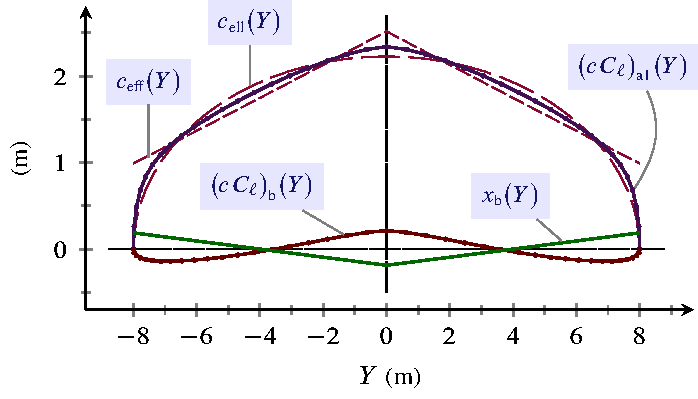
\includegraphics[width=0.80\textwidth]{Chapter_2/pitching_moment_two/wing_Cmac_2_loading_drawing.pdf}%
  \caption{\finalhyphendemerits=1000
           Wing assigned in the examples~\ref{example:Wing:Cmac:A} and~\ref{example:Wing:Cmac:B}.
           Additional loading diagrams $(cC_\ell)_\mathrm{a1}$ and basic loading $(cC_\ell)_\mathrm{b}$ obtained numerically
            (from the Prandtl's Lifting Line Theory)
            and law $x_\mathrm{b}(Y)$ of the basic loading arms.}
  \label{fig:Wing:Cmac:Results:BA}%
\end{figure}


%-----------------------------------------------------------------------------------------------
\begin{figure}[t]%[H]%[!htbp]
  %\centering
  %\checkoddpage
  %\centering
    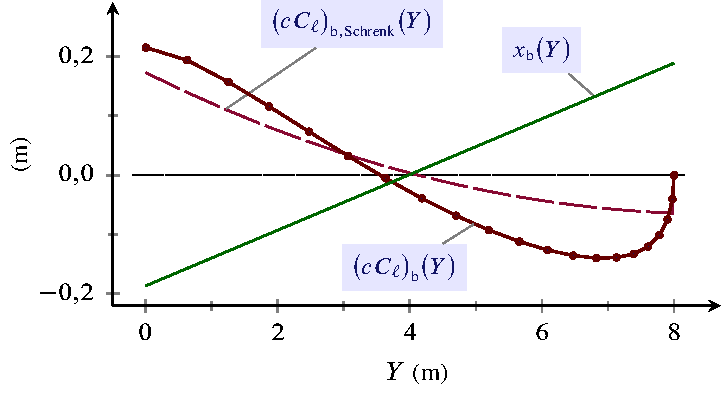
\includegraphics[width=0.80\textwidth]{Chapter_2/pitching_moment_two/wing_Cmac_2_loading_drawing_2.pdf}%
  \caption{\finalhyphendemerits=1000
           Wing assigned in the examples~\ref{example:Wing:Cmac:A} and ~\ref{example:Wing:Cmac:B}.
           Detail of the figure~\ref{fig:Wing:Cmac:Results:BA}.
           Basic loading diagram$(cC_\ell)_\mathrm{b}$ obtained numerically
            with the Lifting Line Theory
         and approximate basic loading $(cC_\ell)_\mathrm{b,Schrenk}$ obtained concurrently
            the application of the Schrenk engineering method for the additional loading
           (see also the figure~\ref{fig:Wing:Cmac:Results:A}).}
  \label{fig:Wing:Cmac:Results:BB}%
\end{figure}
%-----------------------------------------------------------------------------------------------
\begin{figure}
  [t]%[H]%[!htbp]
  %\centering
  %\checkoddpage
  %\centering
    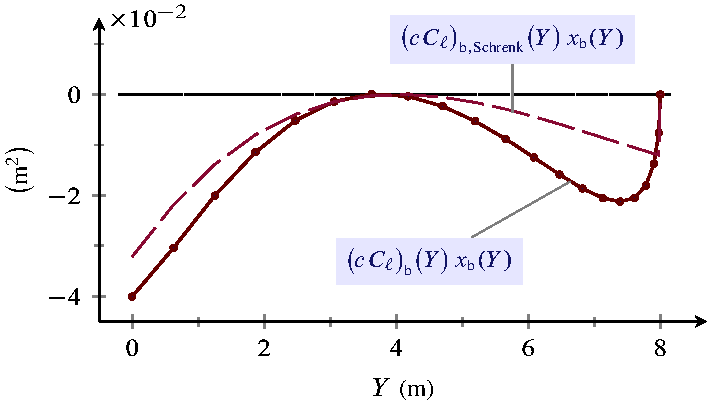
\includegraphics[width=0.80\textwidth]{Chapter_2/pitching_moment_two/wing_Cmac_2_loading_drawing_3.pdf}%
  \caption{\finalhyphendemerits=1000
         Wing assigned in the examples~\ref{example:Wing:Cmac:A} and ~\ref{example:Wing:Cmac:B}.
          Diagram of the two product functions $(cC_\ell)_\mathrm{b}(Y)\,x_\mathrm{b}(Y)$ 
          and $(cC_\ell)_\mathrm{b,Schrenk}(Y)\,x_\mathrm{b}(Y)$
           (see figure~\ref{fig:Wing:Cmac:Results:BC}).
           The integral of these functions allows to estimate the contribution
           \smash{$C_{\mathcal{M}_\mathlarger{\mathrm{ac,b}}}$} to the coefficient
            of pitching moment \smash{$C_{\mathcal{M}_\mathlarger{\mathrm{ac}}}$}
      of the wing around its aerodynamic center.
  }
  \label{fig:Wing:Cmac:Results:BC}%
\end{figure}%
\end{document}
